%%%%%%%%%%%%%%%%%%%%%%%%%%%%%%%%%%%%%%%%%%%%%%%%%%%%%%%%%%%%%%%%%%%
% Background
% Team:
% Wolverine
% Members: 
% Eric Lee, Jacky Wu, Karthick Mani, 
% Eric Chang, Dexter Chen, Peter Chen
% Relative files:
% Team_Wolverine.tex, Team_Wolverine_Compile.tex, Library.bib, WolverineChart.png
% Note:    
% Do not compile this file compile Main.tex to get the pdf file instead.
%%%%%%%%%%%%%%%%%%%%%%%%%%%%%%%%%%%%%%%%%%%%%%%%%%%%%%%%%%%%%%%%%%%
	
\subsection{Information retrieval of existing database}
Author: Eric Lee, Jacky Wu, Karthick Mani, Eric Chang, Dexter Chen, Peter Chen, Kenvin Lo

Aim of this article is to give a brief idea of a database which is about to develop for the purpose of downloading the articles from open access databases using web crawler or web robot. And setting up a system that can allow the users to access the data in our database. we like to separate the article into 6 subsection based on their features, fallowed by then suggestions based on each feature. 


\subsubsection*{Database Management Systems}


A database management system (DBMS) is a computer software application that interacts with the user, other applications, and the database itself to capture and analyze data. Well-known DBMSs include MySQL, PostgreSQL, Microsoft SQL Server, Oracle, Sybase and IBM DB2. And they can support different kinds of databases.


\paragraph{1. Object-oriented database}
An object-oriented database (OODBMS) is a kind of database management 	system.\cite{WiKiauthor2013} The information in the database is represented as objects as used in object-oriented programming.

Because of the tighter integration with object-oriented language, the programmer is easier to maintain consistency with the same representation in both OODBMS and programing language.

Although relational databases which is table-oriented might be similar to object-oriented databases, But they are actually different. Object-oriented database supports objects, classes and inheritance in database schemas and query language.
There are many advantages for OODBMS compared to relational database management system(RODBMS) such as the performance, flexibility, and development cost.

And OODBMS also have some disadvantages, the \cite{Systems2010} have mantion 3 disadvantage for OODBMS. First, because the usage is forced to be similar with object-oriented language. This make maintaining and evolving is  difficult. Second, the technic for store complex type of information take additional computational resources. Third, lack of a standard data model leads to design errors and inconsistencies.


\paragraph{2. Relational database}
A relational database is the most popular database used in the world. They can organize data into one or more tables of columns and rows, with a unique key identifying each row. Rows are also called records or tuples. Generally, each table represents one "entity type" (such as customer or product). The rows represent instances of that type of entity (such as "Lee" or "iPhone 6") and the columns representing values attributed to that instance (such as address or price).

Because of the method of the organization of data, relational database is much easier to understand and is flexible for you to manipulate the data. Besides SQL is easy in the relational database approach. For data organized in other structure the query language either becomes complex or extremely limited in its capabilities. However, once the attributes of data become more and more, you'll need a large amount of table to store your information. Therefore, the performance of relational database will decrease obviously.


\paragraph{3. Graph database}
Graph database uses graph structures for semantic queries with nodes,  edges and properties to represent and store data. Most graph databases are NoSQL in nature and store their data in a key-value store or document-oriented database. Graph databases are a powerful tool for graph-like queries, for example computing the shortest path between two nodes in the graph. Other graph-like queries can be performed over a graph database in a natural way.

Compare to relational databases, there are several advantages. Graph database are often faster for associative data set and map more directly to the structure of object-oriented applications. They can scale more naturally to large data sets as they do not typically require expensive join operations. As they depend less on a rigid schema, they are more suitable to manage ad hoc and changing data with evolving schema.

And graph database have also some disadvantages, relational database are typically faster at performing the same operation on large numbers of data elements. Finally, we want to take one example of graph database: AllegroGraph. 

Because of our lack of the experience of building a database, we think it is important for us to choose a database which is easy to learn and convenience to solve problems we may encounter. Furthermore, it seems relational database is the most capable database which can handle large data among them. Therefore, relational database is our choice.


\subsubsection*{Administrator}
The key feature which binds the relationship between user and administrator. Administrator's point of view, we like to give the best product to the end user. On the other hand, users strive to have convenient searching engine to find what they want at ease. For this purpose, I'm pressure to show two suggestions for enhancing the relationship between users and developer. First, setting up a word-ranking system. When user search for something with specific keyword, such as stem cell in medical area. In this moment, the word-ranking system will help the user by giving some suggested keywords. Of course, the word-ranking systems are developed based on users' searches and expert's suggestions to change the key words. This makes the system trust worthy.
 
Secondly, building up a space in the database and allowing the user to change /edit the space based on their preference. The idea is referenced from well-known database, Wikimedia. It's so called "personalized searching".  By doing this, it would help user idealize their views on the system to what they want and suggest administrator the service which clients really want. It would lead to a win-win situation. 
	
	
\subsubsection*{Web Crawler}
The web crawler is algorithm that has ability to process the data quickly and accurate to update a very large amount of data which are constantly being updated.\cite{Liu2012} It starts with a list of URL to visit, called the seeds. As crawler visits these URL, it identifies all the hyper links in the page and adds them to the list of URL to visit, called the crawl frontier. URL from the frontier is recursively visited according to a set of policies. If the crawler is performing archiving of websites, it copies and saves the information as it goes. The archives are usually stored in such a way they can be viewed, read and navigated as they were on the live web, but are preserved as 'snapshots'.\cite{Du2013} We need to build up a web crawler to automatically visit a list of web page. Then find out which link in the page is valuable to download into our database.
	
	
\subsubsection*{User account}
One of the the main issue is how to create a user account that can connect between user and database. But the more important thing is to make sure database will not collapse by user who is not allowed to access to core part of database. 
 To protect the database system security and privilege, this study introduces two methods for user account, principle of least privilege and role-based access control respectively. The principle of least privilege, also known as the principle of minimal privilege, means giving a user account only those those privileges which are essential to that user's work \cite{PrincipleLeastPrivilege}. The role-based access control is a policy neutral access control mechanism defined around privileges and roles. It can implement discretionary access control (DAC) or mandatory access control (MAC). The role-based access control is very easy to do user assignments as the components of this policy, such as role-permissions, etc. That is why it sometimes referred to as role-based security \cite{RoleBasedAccessControl}. The information and resources would not in danger due to these two methods will filter user depend on their authority and only allow the legitimate user to access. 
	
	
\subsubsection*{User Interface}
Understanding the types of visualizations people create by themselves for personal use. As part of this recent direction, we have studied a large collection of whiteboards in a research institution, where people make active use of combinations of words, diagrams and various types of visuals to help them further their thought processes. Our goal is to arrive at a better understanding of the nature of visuals that are created spontaneously during brainstorming, thinking, communicating, and general problem solving on whiteboards.\cite{Blascheck2016} We use the qualitative approaches of open coding, interviewing, and affinity diagramming to explore the use of recognizable and novel visuals, and the interplay between visualization and diagrammatic elements with words, numbers and labels. We discuss the potential implications of our findings on in- formation visualization design. Combining the advantage of visual thinking new standard of data processing, that visual nature of computers can challenge the first generation of hackers, An icon is an image, picture, or symbol representing a concept.\cite{Szpunar2010}
	
	
\subsubsection*{Data Storage and Search Methods}
The organization of data inside a database management system(DBMS) and retrieval methods is based on the database storage structure such as tables and indexes. There are several types of database storage structure such as XML, a textual data format. This advantage is self-describing and flexible in organizing data.\cite{ISI:000253400700005}Several considerations of data storage include right space allocation techniques, data compression techniques (if necessary), security and encryption and the access path to retrieve the data. Therefore, DBMS software will provide some method to optimize and minimum storage space of a database.
	
\begin{figure*}[h]
	\begin{center}
		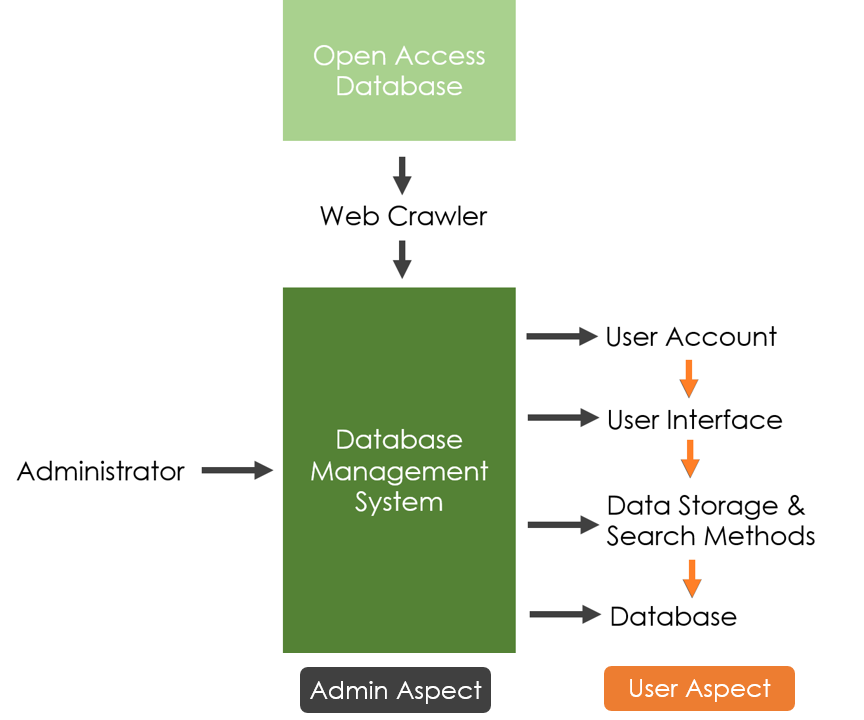
\includegraphics[scale=0.4]{WolverineChart}
	\end{center}
	\caption{Structure of our system}
	\begin{center}
		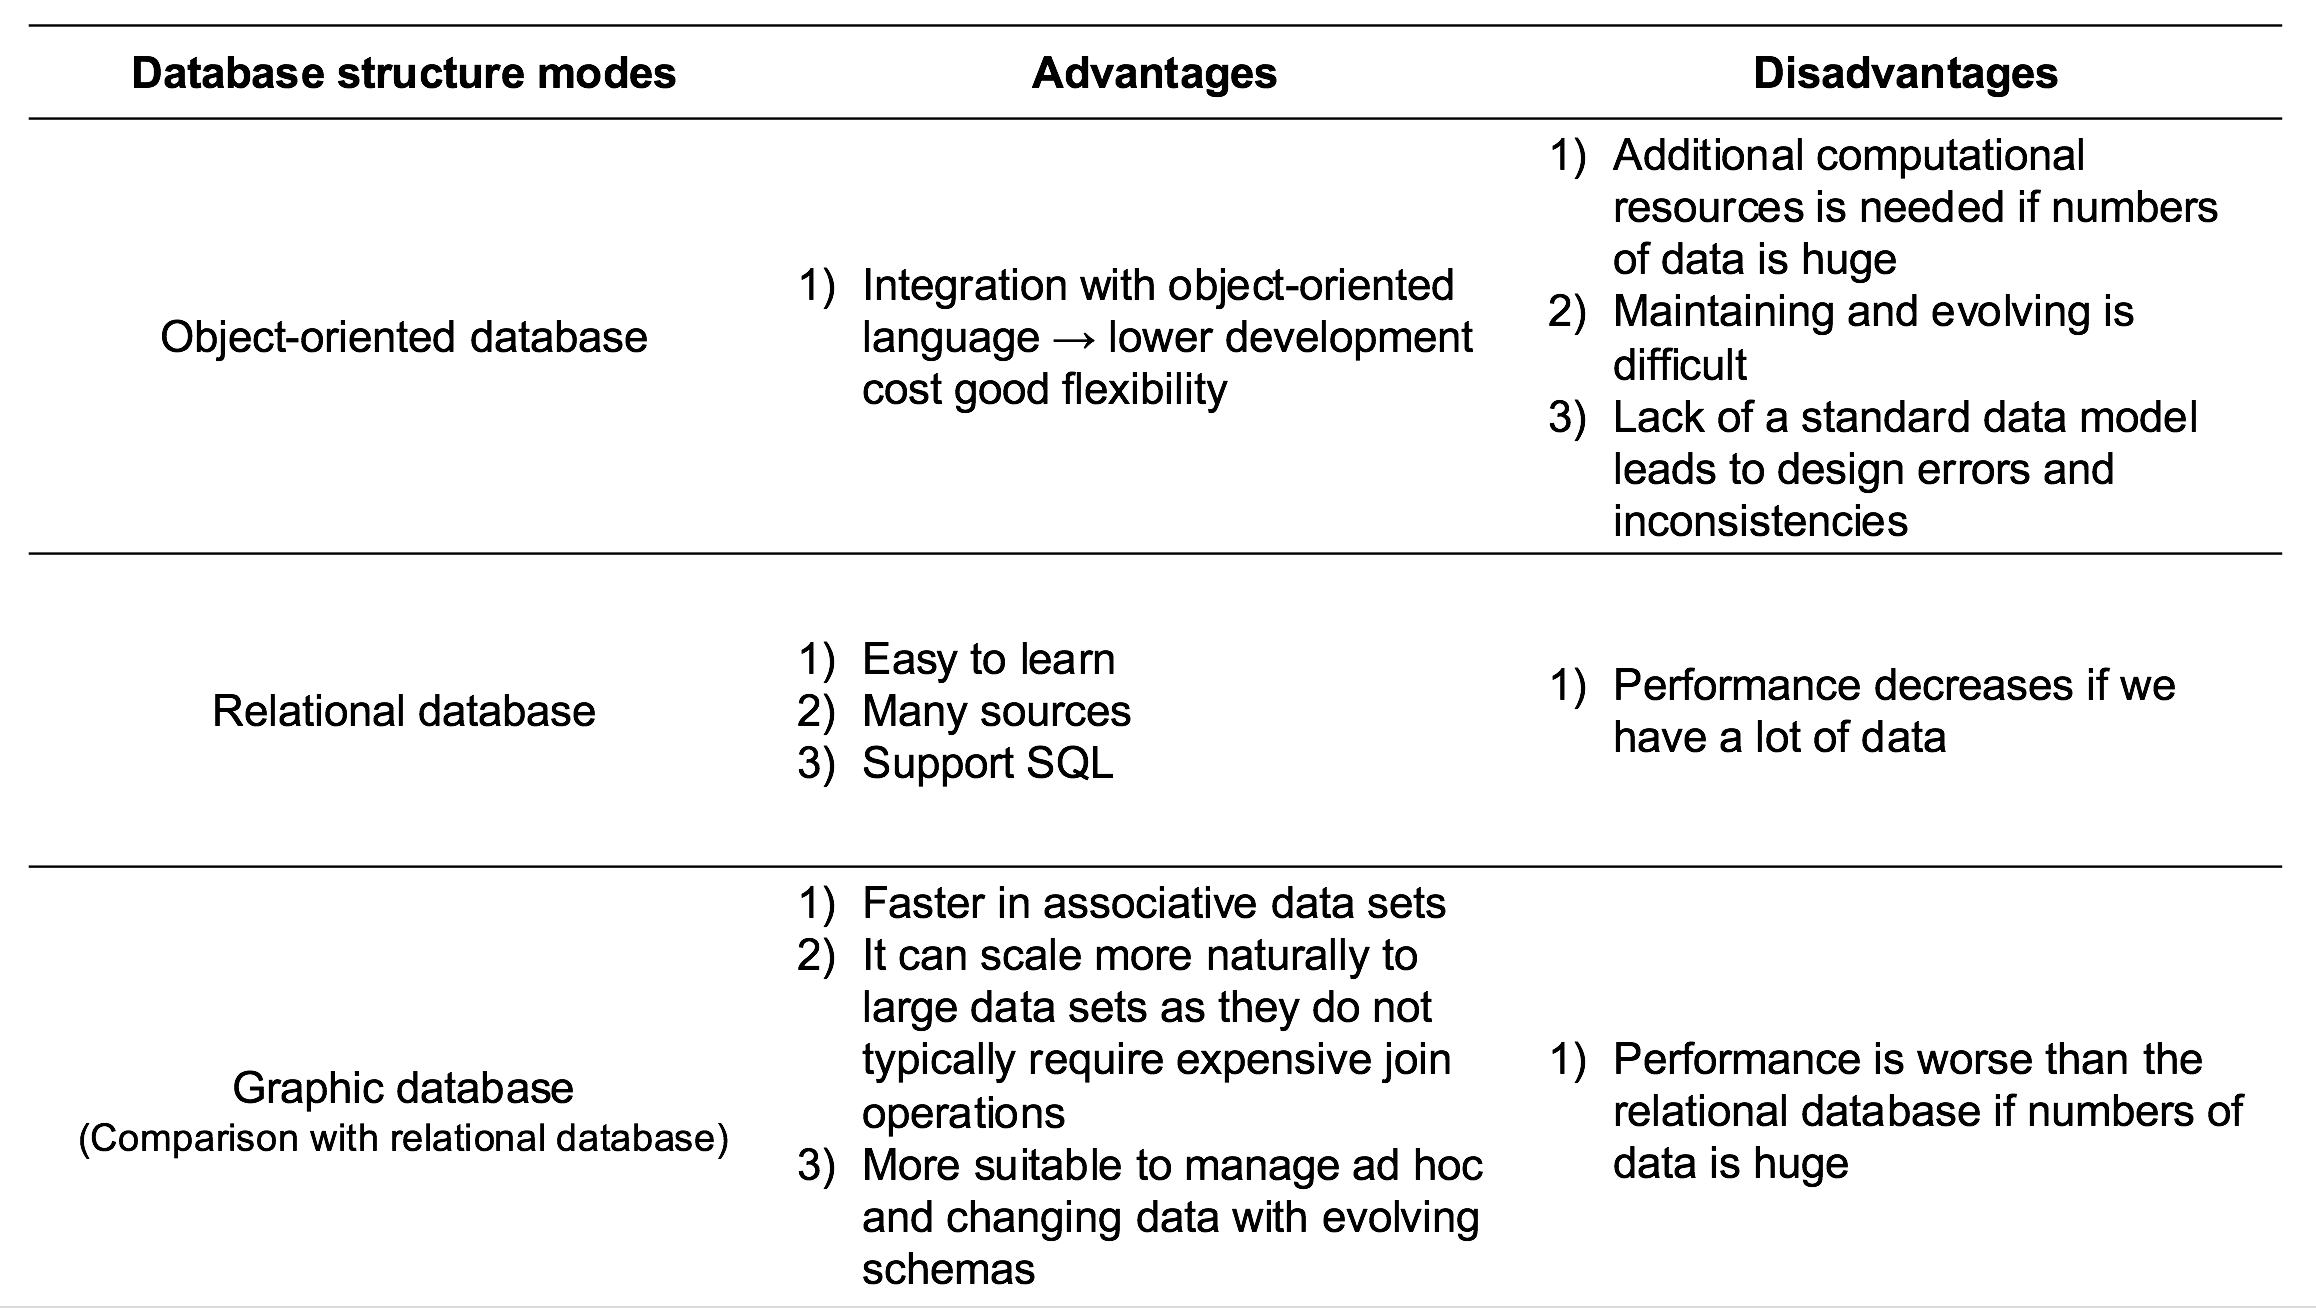
\includegraphics[scale=0.3]{WolverineChart2}
	\end{center}
	\caption{Database structure modes}
\end{figure*}
\clearpage
